\documentclass{article}
    \usepackage[utf8]{inputenc}
    \usepackage{graphicx}
    
    \title{Assignment 1}
    \author{Rajbir Malik \\ 2017CS10416}
    
    \begin{document}
    
    \maketitle
    
    \begin{center}
    \Large{\underline{I. Report on \textbf{Geohash}}}
    \end{center}
    
    \subsection*{Overview}
    Geohashing is method for mapping the locations on earth to strings. It uses Z-ordering for ordering the next division. It, thus, forms a data structure which divides earth into buckets of grid shape, using z-ordering.
    
    \subsection*{Terms Involved}
    It uses a base-32 mapping and divides each section into 32 similar subsections which are connected (and numbered) as per the \emph{Morton Order}.\\\\
    The literals present in the base 32 representation are:
    \begin{center}
        \begin{tabular}{|c|c||c|c|}
             \hline
             No. & Representation & No. & Representation\\
             \hline
             0 & 0 & 16 & h\\
             \hline
             1 & 1 & 17 & j\\
             \hline
             2 & 2 & 18 & k\\
             \hline
             3 & 3 & 19 & m\\
             \hline
             4 & 4 & 20 & n\\
             \hline
             5 & 5 & 21 & p\\
             \hline
             6 & 6 & 22 & q\\
             \hline
             7 & 7 & 23 & r\\
             \hline
             8 & 8 & 24 & s\\
             \hline
             9 & 9 & 25 & t\\
             \hline
             10 & b & 26 & u\\
             \hline
             11 & c & 27 & v\\
             \hline
             12 & d & 28 & w\\
             \hline
             13 & e & 29 & x\\
             \hline
             14 & f & 30 & y\\
             \hline
             15 & g & 31 & z\\
             \hline
        \end{tabular}
    \end{center}
    
    \subsection*{Method}
    Each Block is Divided into 32 Sets as Follows:\\
    \begin{center}
        \begin{tabular}{||c|c|c|c|c|c|c|c||}
        \hline
        \hline
        b & c & f & g & u & v & y & z\\
        \hline
        8 & 9 & d & e & s & t & w & x\\
        \hline
        2 & 3 & 6 & 7 & k & m & q & r\\
        \hline
        0 & 1 & 4 & 5 & h & j & n & p\\
        \hline
        \hline
        \end{tabular}
    \end{center}
    \subsection*{}
    The above division follows z-ordering. The division of Earths map looks like:\\ \\
    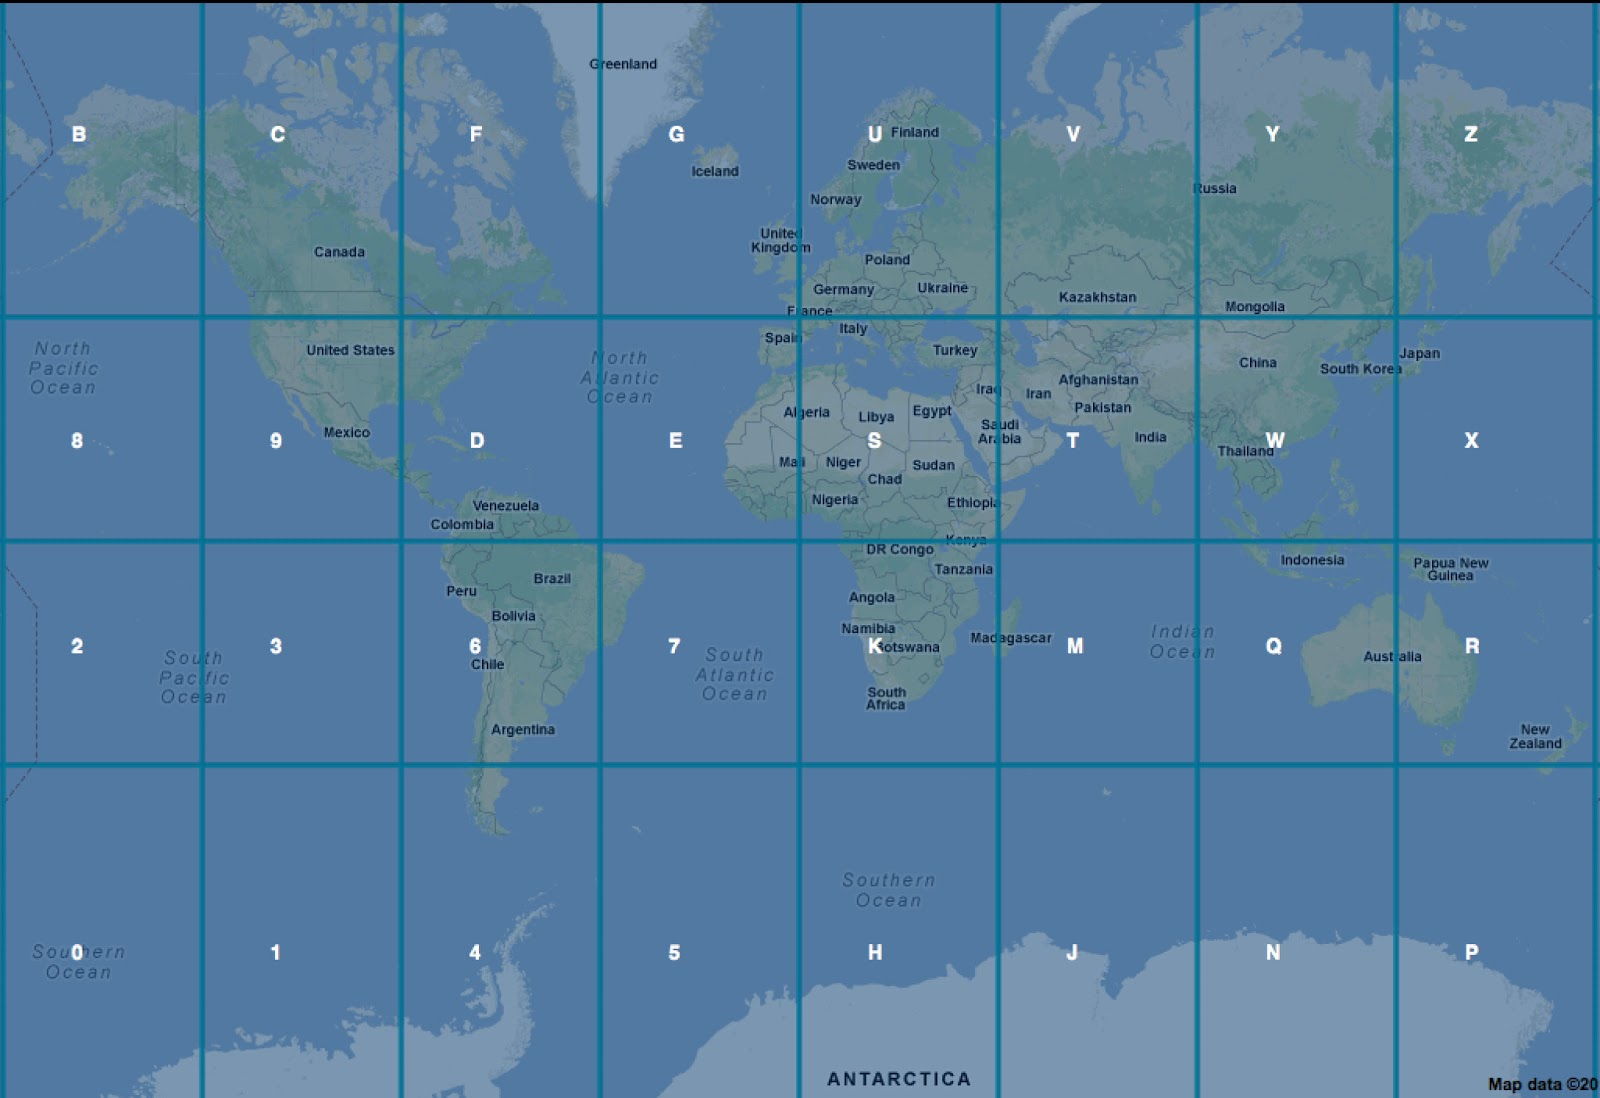
\includegraphics[scale=.25]{./Earth.png}
    
    \subsection*{}
    \paragraph{}
    Now, to get the hash of a particular position (or a region), we enter the region in the above division that contains it. This way all the locations in that particular region will have the same first literal in hash, that is, the location of that region. The next literal would be the position of division in the first region. This we may get to the correct position till arbitrary precision.
    \par 
    
    \pagebreak
    
    \paragraph{}
    This method gives us some amazing and useful properties:
    \begin{itemize}
        \item \emph{Arbitrary Precision}
        \\We could go till any level of division. This would give us a long hash, with the length of hash being the total levels we have gone.
        \item \emph{Size Control}
        \\The size of hash is proportional to the precision of location. We could gradually remove the some literals from the hash to get the location, with some gradual decrease in precision.
        \item \emph{Relation with neighbours}
        \\The neighbours will have very similar GeoHash. Thus we could after seeing the literal could comment on the distance to a good level of approximation. \\ 
    \end{itemize}
    \par
    
    \underline{\emph{The length of hash (the number of divisions) and size of region are related as}}
    \begin{center}
        \begin{tabular}{|c||c||c|}
             \hline
             Hash Length & Width & Length \\
             \hline
             1	& 5,000km	&	5,000km \\
             \hline
             2	& 1,250km	&	625km \\
             \hline
3	& 156km	&	156km \\
\hline
4	& 39.1km	&	19.5km \\
\hline
5	& 4.89km	&	4.89km \\
\hline
6	& 1.22km	&	0.61km \\
\hline
7	& 153m	&	153m \\
\hline
8	& 38.2m	&	19.1m \\
\hline
9	& 4.77m	&	4.77m \\
\hline
10	& 1.19m	&	0.596m \\
\hline
11	& 149mm	&	149mm \\
\hline
12	& 37.2mm	&	18.6mm \\
             \hline
        \end{tabular}
    \end{center}
\paragraph{From the above table, we can conclude two things}
\begin{itemize}
    \item \emph{Odd numbered regions are squares and Even numbered are rectangles with 2:1 ratio. This is done to ensure easy divsion of earth.}
    \item \emph{We can achieve very reasonable precision (~1m) within the hash of length 10.}
\end{itemize}

\pagebreak

\subsection*{Limitations \small{(When Working in Proximity Analysis)}}
It has two major flaws when using it for proximity analysis (getting the idea of distance or nearness of two positions given their geohashes).
\paragraph{ - Edge Cases} 
     One can observe that positions on the edges of a divsion have a drastically different geohash compared to its immediate neighbour in the other division. This could lead to problems as these two despite being near have quite different geohashes.
\paragraph{ - Non Linearity}
    This suggests that, since earth is spherical, the direct angular relation between distances with longitude and latitudes won't be possible. Thus geohashes can't directly give distance between to positions.

    
\subsection*{Summary}
Summarizing we can say that geohashing is a great way to represent positions on earth. Its flexibility and simplicity allows to target any location on earth. It also gives us idea of relative positions. Thus, it is of great use!

\pagebreak
    
    \begin{center}
    \Large{\underline{II. Computation of Geohashes}}
    \end{center}

\subsection*{Overview}
We are asked to compute the geohash of
\begin{enumerate}
    \item \emph{IIT Delhi Main Building}
    \item \emph{Connaught Place}
\end{enumerate}
\underline{Now their respective Latitudes and Longitutes are :}
\begin{center}
    \begin{tabular}{||c||c|c||}
    \hline
        Location & Latitude & Longitude \\
    \hline
        IITD Main Building & 28.54497 & 77.19252\\
    \hline
        Connaught Place & 28.6331 & 77.217\\
    \hline
    \end{tabular}
\end{center}
\subsection*{Computation}
Now we can compute the geohash from the map, going to the suitable section in each division, till we get to desired precision.
\begin{center}
    \begin{enumerate}
        \item \textbf{t} - Contains Most of India
        \item \textbf{tt} - Contains Most of North India
        \item \textbf{ttn} - Contains Most of Haryana and Delhi
        \item \textbf{ttnf} - Contains South and Central Delhi
    \end{enumerate}
\end{center}
Now, this position contains both the desired locations. But, after this location both get separated in different locations. \\ \\

Continuing in Similar Fashion, we are able to get the locations to our desired level of precision...
\begin{itemize}
    \item IIT Delhi Main Building - \textbf{ttnfks3}
    \item Connaught Place - \textbf{ttnfvh}
\end{itemize}
    \end{document}
    